\documentclass[a4paper,openright,12pt]{report}
\usepackage[spanish]{babel} 
\usepackage{multirow}
%\usepackage[latin1]{inputenc}
\usepackage[utf8]{inputenc}
\usepackage{graphicx}
\usepackage{lmodern}
\usepackage{listings}
\usepackage{color}
\usepackage{fancyhdr}
\usepackage{hyperref}
\usepackage[left=2.5 cm,right=2cm,top=2.5 cm,bottom=3cm]{geometry}

\usepackage{Sweave}
\begin{document}
\Sconcordance{concordance:Examen.tex:Examen.Rnw:%
1 13 1 1 0 106 1 1 4 36 0 1 2 5 1 1 6 4 0 1 2 2 1 1 6 4 0 1 2 2 1 1 6 4 %
0 1 2 2 1 1 6 4 0 1 2 2 1 1 5 4 0 1 2 2 1 1 5 4 0 1 2 2 1 1 4 10 0 1 2 %
4 1}



\pagestyle{fancy}
\renewcommand{\headrulewidth}{0pt}
\bigskip
\bigskip


{\setlength{\arrayrulewidth}{0.5mm}
\begin{tabular}{p{2 cm} | p{10
cm} p{3 cm}}
\multirow{3}{2cm}{\Large{
\includegraphics[width=1.9 cm]{unloja}}} 
&\Large{\textbf{UNIVERSIDAD}}&\multirow{3}{2cm}{\Large{
\includegraphics[width=3 cm]{logo13}}}\\

& \Large{\textbf{NACIONAL}}& \\
& \Large{\textbf{DE LOJA}}&\\
\end{tabular}
\bigskip
\bigskip

\begin{flushleft}


\raggedright{ 
\small{\textit{\textbf{Área de la Energ?a, las Industrias y los Recursos Naturales No Renovables}}}
}
\thinspace
\rule{1\textwidth}{0.04cm} 
\thinspace
\raggedleft{ 
\Large{\textsc{Carrera de Ingenier?a en Sistemas}}}
\end{flushleft}
\bigskip
\bigskip
\bigskip
\bigskip
\bigskip

\begin{center}
\begin{Huge}
\textbf {EXAMEN DE ANÁLISIS DE SOFTWARE}
\end{Huge}
\bigskip
\bigskip
\bigskip
\bigskip
\bigskip
\bigskip
\bigskip


\begin{LARGE}
\end{LARGE}
\small{\textsc{Sexto A}}\\
\bigskip
\end{center}
\bigskip
\bigskip


\begin{flushleft}
\textit{\textbf{Autores:}}
\begin{itemize}
\renewcommand{\labelitemi}{$\diamond$} 
\item José Angel Loja       -      \href{http://www.iralis.org/?q=node%2F10&paso=10&letra=L&id=5186/}{ECINF5186}
\end{itemize}
\bigskip
\bigskip
\end{flushleft}
\thinspace
\bigskip

\begin{flushleft}
\textit{\textbf{Tutor:}}
\begin{itemize}
\renewcommand{\labelitemi}{$\diamond$} 
\item \href{http://www.iralis.org/?q=node%2F10&paso=10&letra=O&id=4796}{ECINF5187}
\end{itemize}
\begin{center}\href{http://creativecommons.org/choose/}{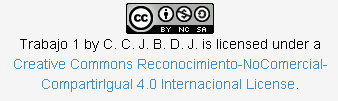
\includegraphics[width=8cm]{Licencia}}\end{center} 
\bigskip
\bigskip
\end{flushleft}
\thinspace
\bigskip

\newpage
\begin{center}
\begin{Huge}
\textbf {PARTE b}\\
\end{Huge}
\end{center}
Desarrollar las siguientes actividades a partir del dataset Titanic (Data sets in package 'datasets'), y de la Ingeniería del Software:\\

\begin{itemize}
\item \textbf{¿Es aplicable la ingeniería de software cuando se elaboran webapps? Si es así, ¿cómo puede modificarse para que asimile las características únicas de éstas?}\\

Si es aplicable la Ingenieria de software en el desarrollo de webapss. Pero se deberia modificar el proceso de calidad de software, ya que se lo deberia hacer durante todo el ciclo de desarrollo. Tambien se deberia hacer una modificacio en el mantenimiento de software, para de esta manera se pueda tener una software mas mantenible.

\item \textbf{Un breve descripción del dataset Titanic:}\\

A inicios de la de la decada anterior, se sucitó el accidetnet del titanic. Muchos estudios datan información acerca de este suceso. Cientos de investigadores, nos tratan de dar cifras exactas de cuantos fueron los fallecidos en este accidente.
El el dataset Titanic, se datan las cifras de víctimas que hubieron en el hundimienton del titanic. Están agrupados en columnas dependiendo la clase donde viajaban, en la columna Class. En la columna Sex, están el sexo al que pertenecian. En la columna Sorvived, nos indica si sobrevieron o no. Y en la columna Freq, está la cantidad de personas que fallecieron o que sobrevivieron

\item \textbf{Mostrar el dataset}\\
Para mostrar el dataset, lo descargamos y lo abrimos desde el escritorio
\begin{Schunk}
\begin{Soutput}
   Class    Sex   Age Survived Freq
1    1st   Male Child       No    0
2    2nd   Male Child       No    0
3    3rd   Male Child       No   35
4   Crew   Male Child       No    0
5    1st Female Child       No    0
6    2nd Female Child       No    0
7    3rd Female Child       No   17
8   Crew Female Child       No    0
9    1st   Male Adult       No  118
10   2nd   Male Adult       No  154
11   3rd   Male Adult       No  387
12  Crew   Male Adult       No  670
13   1st Female Adult       No    4
14   2nd Female Adult       No   13
15   3rd Female Adult       No   89
16  Crew Female Adult       No    3
17   1st   Male Child      Yes    5
18   2nd   Male Child      Yes   11
19   3rd   Male Child      Yes   13
20  Crew   Male Child      Yes    0
21   1st Female Child      Yes    1
22   2nd Female Child      Yes   13
23   3rd Female Child      Yes   14
24  Crew Female Child      Yes    0
25   1st   Male Adult      Yes   57
26   2nd   Male Adult      Yes   14
27   3rd   Male Adult      Yes   75
28  Crew   Male Adult      Yes  192
29   1st Female Adult      Yes  140
30   2nd Female Adult      Yes   80
31   3rd Female Adult      Yes   76
32  Crew Female Adult      Yes   20
\end{Soutput}
\end{Schunk}


\item \textbf{¿Cuál es el número total de casos en el dataset?}\\
El número total de casos es el siguiente:\\
\textbf{Niños y Niñas Fallecidos}\\

\begin{Schunk}
\begin{Soutput}
[1] 52
\end{Soutput}
\end{Schunk}

\textbf{Niños y Niñas que Sobrevieron}\\

\begin{Schunk}
\begin{Soutput}
[1] 57
\end{Soutput}
\end{Schunk}

\textbf{Adultos que No Sobrevieron}\\

\begin{Schunk}
\begin{Soutput}
[1] 1438
\end{Soutput}
\end{Schunk}

\textbf{Adultos que Sobrevieron}\\

\begin{Schunk}
\begin{Soutput}
[1] 654
\end{Soutput}
\end{Schunk}

\textbf{Numero Total de Personas que sobrevivieron}\\

\begin{Schunk}
\begin{Soutput}
[1] 711
\end{Soutput}
\end{Schunk}

\textbf{Numero Total de Casos:}\\

\begin{Schunk}
\begin{Soutput}
[1] 2201
\end{Soutput}
\end{Schunk}

\textbf{Estadísticas:}\\

\begin{Schunk}
\begin{Soutput}
  Class       Sex        Age     Survived      Freq       
 1st :8   Female:16   Adult:16   No :16   Min.   :  0.00  
 2nd :8   Male  :16   Child:16   Yes:16   1st Qu.:  0.75  
 3rd :8                                   Median : 13.50  
 Crew:8                                   Mean   : 68.78  
                                          3rd Qu.: 77.00  
                                          Max.   :670.00  
\end{Soutput}
\end{Schunk}
\end{itemize}


\end{document}

